\documentclass[english, 11pt]{article}
\usepackage{notes}

\newcommand{\thiscoursecode}{TRIUMF SEMINAR NOTES}
\newcommand{\thiscoursename}{Student Seminars}
\newcommand{\thisprof}{Staff}
\newcommand{\me}{Jason Liu}
\newcommand{\thisterm}{(Winter) 2014}
\newcommand{\website}{lithium11.com}

% Headers
\chead{\thiscoursename}
\lhead{\thisterm}

% Title
\newcommand{\notefront} {
\pagenumbering{roman}
\begin{center}

{\ttfamily \url{\website}} {\small}

\textbf{\Huge{\noun{\thiscoursecode}}}{\Huge \par}

{\large{\noun{\thiscoursename}}}\\ \vspace{0.1in}

  {\noun \thisprof} \ $\bullet$ \ {\noun \thisterm} \ $\bullet$ \ {\noun {Jason Liu}} \\

  \end{center}
  }

% Begin Document
\begin{document}

  % Notes front
  \notefront
  % Table of Contents and List of Figures
  \tocandfigures
  % Abstract
  \doabstract{These notes are intended as a resource for myself; past, present, or future students of this course, and anyone interested in the material. The goal is to provide an end-to-end resource that covers all material discussed in the course displayed in an organized manner. If you spot any errors or would like to contribute, please contact me directly.}


% Vijay K. Verma
    \section{Project Managment}
      The goal of this workshop is to do a brief overview of PMI, project management and process groups. Balancing project requirements and influence of the uncertainty. 

    \subsection*{What is Unique in Scientific Organizations}
      Unlike some pure engineering paths, there is more uncertainty in research. We have limited funding with bleeding edge techonology. Moreover, we have specialized people and skill mixes along with special constraints like radiation, dose limits etc.. Special challenges also occur like regulations, international collaborations and politcal ones.

    \subsection*{Learning Objectives}
      \begin{itemize}
        \item What is \nameref{project management}
        \item PMBOK knowledge areas and constraints
        \item Project management processes
        \item \nameref{plc}
        \item \nameref{pmbok}
      \end{itemize}

      \begin{defn}[Project]\label{project}
        A temporary endeavor undertaken to unique project or service.
      \end{defn}

      \begin{defn}[Project Management]\label{project management}
        Application of knowledge, skills, tools and techniques to project activies in order to meet or exceed stakeholder needs and expectations from a \nameref{project}. We need to understand what people want without them knowing. They will want it, so deliver.
      \end{defn}

    \subsection{Project Manager}
      slides(49, 50, 51)

    \subsection{Processes of PMI}
      \begin{enumerate}
        \item Initiating: Authorizing the project. Spending resources to start.
        \item Planning: Defining and refining objectives, select best course of action.
        \item Executing: Coordnating and intergrating people to carry out plan.
        \item Monitoring and Control: Measure progress, identify variance and cause to take corrective actions.
        \item Closing: Formalize acceptance of project and bring to orderly end.
      \end{enumerate}

    \subsubsection*{Crazies}
      People and money and others all effect the project. We also need strong a strong champion. Things like priorities and stakeholders keep changing. We need to figure out the network and get things done in the end. Management only hears what they want to hear. They can't hire or fire any thing. You need to give conditions that lead to success. You can't say no.

    \subsubsection{PMBOK Definitions}\label{pmbok}

      \begin{defn}[Project Scope]\label{scope}
        The work that needs to be accomplished to deliver a product, service, or result with the specified features and functions.
      \end{defn}

      \begin{defn}[Project Life Cycle]\label{plc}
        Collection of sequencial project phases whos name and number are determined by the control needs of the organizations involved in the project. It changes by the industry.
      \end{defn}

      \begin{defn}[Work Breakdown Structure]\label{wbs}
        A deliverable-oriented grouping of the project elements which organizes and defines the total scope of the project.It helps organize the total scope of the project. Divide work into stand-alone. Often in the form of a tree diagram.
      \end{defn}

      \begin{defn}[Organization Breakdown Structure]\label{obs}
        Project organization relating work packages to organizational units or people responsible. Ontop of the tree diagram of \nameref{wbs}, each block refers to the person responsible.
      \end{defn}

      \begin{defn}[Project Phase]\label{project phase}
        A collection of related \nameref{activity}, usually culminating in the completion of a major deliverable
      \end{defn}

      \begin{defn}[Activity]\label{activity}
        An element of work performed during the course of a \nameref{project phase} usually has a duration and expected cost and expected resources requirments, and be subdivided into tasks.
      \end{defn}

      \begin{defn}[Task]\label{task}
        The lowest level of effort on a project, subdivided \nameref{activity}. Ones all tasks are finished, one has achieved a milestore.
      \end{defn}

      \begin{defn}[Milestone]\label{milestone}
        A significant event in the \nameref{project} usually completion of a major.
      \end{defn}

      \subsubsection{Defining Success}
      \begin{itemize}
        \item Accepted by stakeholders and it just either meet or exceed the expectations
        \item Meeting the performance requirement (scope)
        \item On time and in budget
        \item Minimumn shane in scope and does not corpate workflow
      \end{itemize}

      \subsection{Time Management}
        There are some key processes required to ensure timely completion of the projects. We have to {\bf define} the \nameref{activity} that must be performed. We must {\bf sequence} events and identify and document dependencies. We also must {\bf estimate} the number of work periods wich whill be need to complete individual activies. Schedule development and control is also important.

      \subsubsection{Planning Approach?}
        \begin{enumerate}
          \item Define \nameref{scope}
          \item Develop \nameref{wbs}
          \item Develop \nameref{obs}
          \item Prepare Responsbility Matrix
          \item Prepare Project Cost Estimate
          \item Define Quality Requirements
          \item Identify activity sequence and dependencies
          \item Identify the critical path and calculate project duration
          \item Analyse risk
          \item Assemble Project Plan and get Approval
        \end{enumerate}

      \subsubsection{Planning Benefits?}
        IThe benefits of planning this way is that it is an interactive approach to ensure nothing is overlooked. It allows for better communicatoin between stakeholders and it serves as the starting point for project approval. With planning done right, changes in scope and be noted and risks are addressed. By documenting this process, it becomes easier to justify the requirements of the project. \\

      \subsubsection{Statement of Work}
        The following is the contents of what a general statement of work.
        \begin{itemize}
          \item Purpose of Project
          \item Scope Statement
          \item Product Definition (deliverables)
          \item Cost \& Schedule Estimates
          \item Project Organization Stucture
          \item \nameref{ram}
          \item Risks
          \item Assumptions
          \item Project Success Factors
        \end{itemize}
      
      \subsubsection{Responsibility Matrix }\label{ram}

      \begin{exmp}[Software Development]
      This is a Responsibility Assignment Matrix. B - Responsible, A = Accountable, C = Consult, I = Inform.
      \begin{center}
        \begin{tabular}{|l|l|l|l|l|}
          \hline
          ~                  & Kelly & Jason & Jonah & Jake \\ \hline
          Define Requirments & C     & R     & A     & A    \\
          Functional Specs.  & I     & A     & C     & R    \\
          Coding             & I     & C     & R     & A    \\
          Documentation      & C     & R     & A     & I    \\
          Systems Design     & R     & A     & C     & I    \\ \hline
        \end{tabular}
      \end{center}
      \end{exmp}
      
      \subsubsection{Milestones}
        It is often important to define milestones in any project. A time to celebrate completion of a portion of the project. With this in mind, we need to figure out different ways to tracking a project. Bar charts are one way of figure out what needs to be done. They are easy to prepare and update but they can become complex and does not help with the control of the project. One better method to use would be the \nameref{cpm}.

      \subsubsection{Critical Path Method} \label{cpm}
        \begin{defn}[Critical Path] \label{cp}
          The longest path through the network. It has zero float defined by a logical sequence of activities. It may be calculated after the activities have been scheduled. It determines the earliest expected project finish date. 
        \end{defn}

        The \nameref{cp} is essentially a network of tasks. They are ordered in time and can have a parallel structure. the path with the most time is the \nameref{cp} and it has no float. Delays in the \nameref{cp} will cause the project to delay. This method of time management helps us decide where to alocate scare resources.\\

      \subsubsection{Path Techniques}
        There are various techniques we can use to optimize the critical path. If we can use more resources, like staff or equipment, we can start doing jobs in parallel. If we are able to take on more risk, we can fast track and overlap sequencial activities. The main thing we want to do in every case is to maximize compression for least cost.


% Stanley Yen
  \section{Constituents of Nucleons}

  \subsection{Quantum Review}
    There are a few things we must understand abotu quantum physics. Light is a wave because it shows inferferences and it is also a particle by the photoelectric effect.

    \begin{defn}[Photoelectric Effect]\label{pe}
    Light energy comes in packets of size. Where $h$ is Planck's Constant and $f$ is the frequency of light.
      \[ E =hf \]
    \end{defn}

    This is a general property of all matter, not just of light. It is possible to see diffraction patterns made by beams of electrons, neutrons, protons, carbon atoms, and even Buckyballs!

    This is the fundamental principle of wave-particle duality.

    \begin{defn}[De Broglie's Wavelength]
      The wavelength of particle is given by $\lambda = h\cdot p$ where $p$ is the particle's momentum
    \end{defn}

    By \nameref{hup}, the act of measurement disturbs the system being measured.

    \begin{defn}[Uncertainty Principle]\label{hup}
      The uncertainty principle is any of a variety of mathematical inequalities asserting a fundamental limit to the precision with which certain pairs of physical properties of a particle known as complementary variables.
      \[ \sigma_x \sigma_y \leq \hbar/2 \]
    \end{defn}

    In this lectures we shall apply these princples of quantum mechanics to several topics of subatomic physics.

    \begin{itemize}
      \item The size and shapes of nuclei
      \item The energy scale of nuclear processes
      \item The existence of quarks
    \end{itemize}

    \subsection{Sizes and Shapes}

      If we want to see nuclei, we can't just put it under a microscope.The wavelengths of the light used is proportional to it's resolution and visible light is pretty bad in this case. 

      However, if that is the case, how can we possibly see nuclei? The answer is scattering, however, the analogy of bullets through a haystack is not accurate due to the the wave effects of particles on this scale. As mentioned previously, electrons are not only particles but waves as well, when we intercept a beam with nuclei, we will get diffraction pattern of electrons that we can then study. \\ 
      \subsubsection{Experiment}

      When a group of waves hit an object with some sort of internal structure, the points act like a point source of waves. If they are far apart, there will be many peaks. If they are closer together we have a maximum, and if they are a single particle, we get a single wave crest. The nucleus however is not an infinity small point. It is really more like a charge semeared over a volume. However we have a method of using this approximation to get better results.

        \[ S_{spaced} = S_{pointlike} \cdot |\int \rho(r') e^{iqr'}dV'| ^2 \]

      For elastic scattering at angle $\theta q = 2p / \hbar * \sin(\theta θ/2)$

      By measuring the scattering rate at different angles $\theta$, and sampling at different values of $q$, we can map out the square of the Fourier transform.Then apply an inverse Fourier transform to get the nuclear charge density $\rho(r')$
      
      To do this, we have an electron beam collide into target some times the electrons interact with the nucleonsa nd bounce off. We can use a magnetic spectrometer to look at the distribution of electrons post-interaction. By swinging this spectrometer at different angles, we sample the space. \\

      \begin{center}
        [scattering image]
      \end{center}

      \subsubsection{Interpretation -fix}

      When we look at the actual distributions, the largest peak represents the elastic scattering while the rest of the bumps are always inelastic, there the electron happened to excite the nucleous (something inside the nucleous).\\
      Since a small object gives a large diffraction and vise versa, we can calculate use the data to calculate the radius of nuclei. The narrower the diffraction the larger the radius of the nucleous.\\
      If a atom was the size of football stadium, the nucleous would be on the scale of a pea. Yet it it 99.97\% of its mass

    \subsection{Nuclear Energy Scale}

    Similar to electrons, protons and neutrons have shell like structures. However, nuclear energies are very high. This can be explained by the \nameref{hup}. Since nuclei are 45000x smaller than atomic scales, by the \nameref{hup}, since $\Delta x$ is very small, $\Delta p$ is very high. 

    \begin{align*}
      p_n / p_a &= 45000\\
      KE_n / KE_a &= (45000)^2 / 1836 = 1.1\e{6}
    \end{align*}

    \subsection{Quarks}

    Later on the question was posed to whether or not protons and neutrons were the last of the particles. The answer came in the form of using narrower and narrower wavelengths to probe the nucleons furthur. 

    What we can do is shoot electrons at a film of solid hydrogen and see how the protons defract. Back in the day, 1/100 fm was the attainable wavelengths of those electrons, much smaller than the current accepted radius of a proton. This meant that we could definitly have resolution of things smaller than the protons if they were indeed as small we thought they were.\\

    Looking at the diffraction pattern we noticed that it wasn't equal, it wasn't a single crest. Instead it looked similar to our studies of nuclei. The plots showed elastic collisions happening with large amplitudes and a few bumps, signalling inelastic scattering. This pattern meant that there were indeed internal `things' that could be excited. this meant that nucleons could be excited. Moreover, we notice that at very large angles, evidence suggests that there are point like objects inside the proton as the bumps smooth out to supposed point like particles.\\

    Three quarks for muster mark. 

    \section{Nuclear Structures}
        This talk summarizes our knowledge of nuclei and nuclear structure. First there was a brief over of the common units and unit scales and along with definitions if isotopes, isobars, isotones, types of decay and the chart of nucleids. 

      \subsection{Binding Energies}

      \begin{defn}[Binding energy]\label{be}
        Binding energy is the mechanical energy required to disassemble a whole entity into separate parts. A bound system typically has a lower potential energy than the sum of its constituent parts, this is what keeps the system together.$^{[W]}$ 
      \end{defn}

      Recall $e=mc^2$, the main idea here is that the relationship between mass and energy are shared. However, the proportion of scaling is negligable at the macroscopic level. However, at the subatomic level when we bind two particles together, they decrease their energy and therefore decrease their mass. 

      \begin{exmp}[Atomic Mass from Binding]
        \[  m_{atom} = m_{nucleus} + m_{electrons} - \frac{b_{e}}{c^2} \]
      \end{exmp}
      
      Nuclear binding energies however are much larger than atomic binding. In most cases, the atomic binding energy is usually just a tiny correction term that may be omited. In fact, we look at most tabular data you will find that it will be in an atomic energy which we can convert to nuclear by using the correctional terms.\\

      \subsection{Saturation}

      Consider the term $B/A$, it is the average binding energy per nucleon. Emperically, the average $B/A$ is $8 MeV$ (Average of an Average? Yes please!). The plot itself peaks at iron and slowly decreases as the increasing repultion of the protons causes us to pack more and more nuetrons in to introduce enought strong force to balance the electrostatic. This is called the saturation of nuclear forces. 

      \begin{center}\label{plot}
         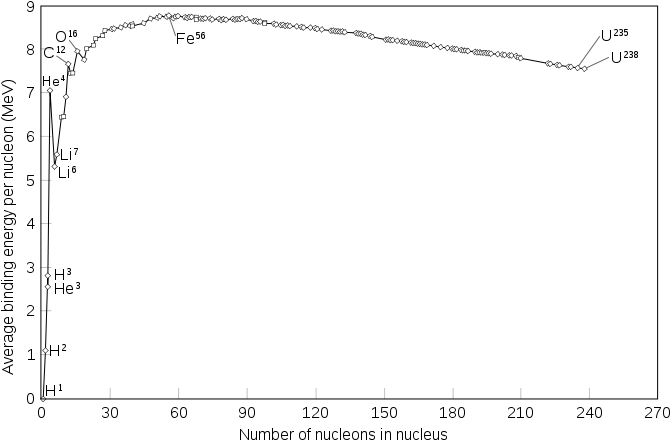
\includegraphics[scale=0.5 ]{../img/ba}
      \end{center}

      \begin{defn}[Saturation of Nuclear forces]\label{sat}
        The nucleus has become large enough that nuclear forces no longer completely extend efficiently across its width. Attractive nuclear forces in this region, as atomic mass increases, are nearly balanced by repellent electromagnetic forces between protons$^{[W]}$
      \end{defn}
     
      At the size individual nucleons only feel a neighbourhood of forces. This indicates that the nuclear binding forces must be short ranged, similar to the forces of a kettle of water; it is the short ranged van der wals forces that hold it together. 
      \\ 
      \[ e_{boil} = e_{binding} \propto A^2_{water} \]

      This is constant due to the short range of the forces. 

      \[ B \propto A^2 \implies B/A  \propto A\]

      This $8 MeV$ is about $1\%$ the total mass of the proton. This means that the mass of a nucleus is nearly $1\%$ smaller than the mass of it's constituent nucleons. Now its not on the order of $10^{-9}$ it is not negligitable. 

      \subsection{Studing the plot (\ref{plot})}

      By looking at the plot from \ref{plot} plot we can learn a lot about nuclear processes. 
      The first peak is related to the production of $He^{4}$ in the sun, which releaes 28MeV per fusion! That part of the plot is where most stars spend their lives. Successive steps take far less energy. This helps us understand other properties of stars by looking at the Hertzsprung-Russell diagram. 

      \begin{center}\label{rus}
         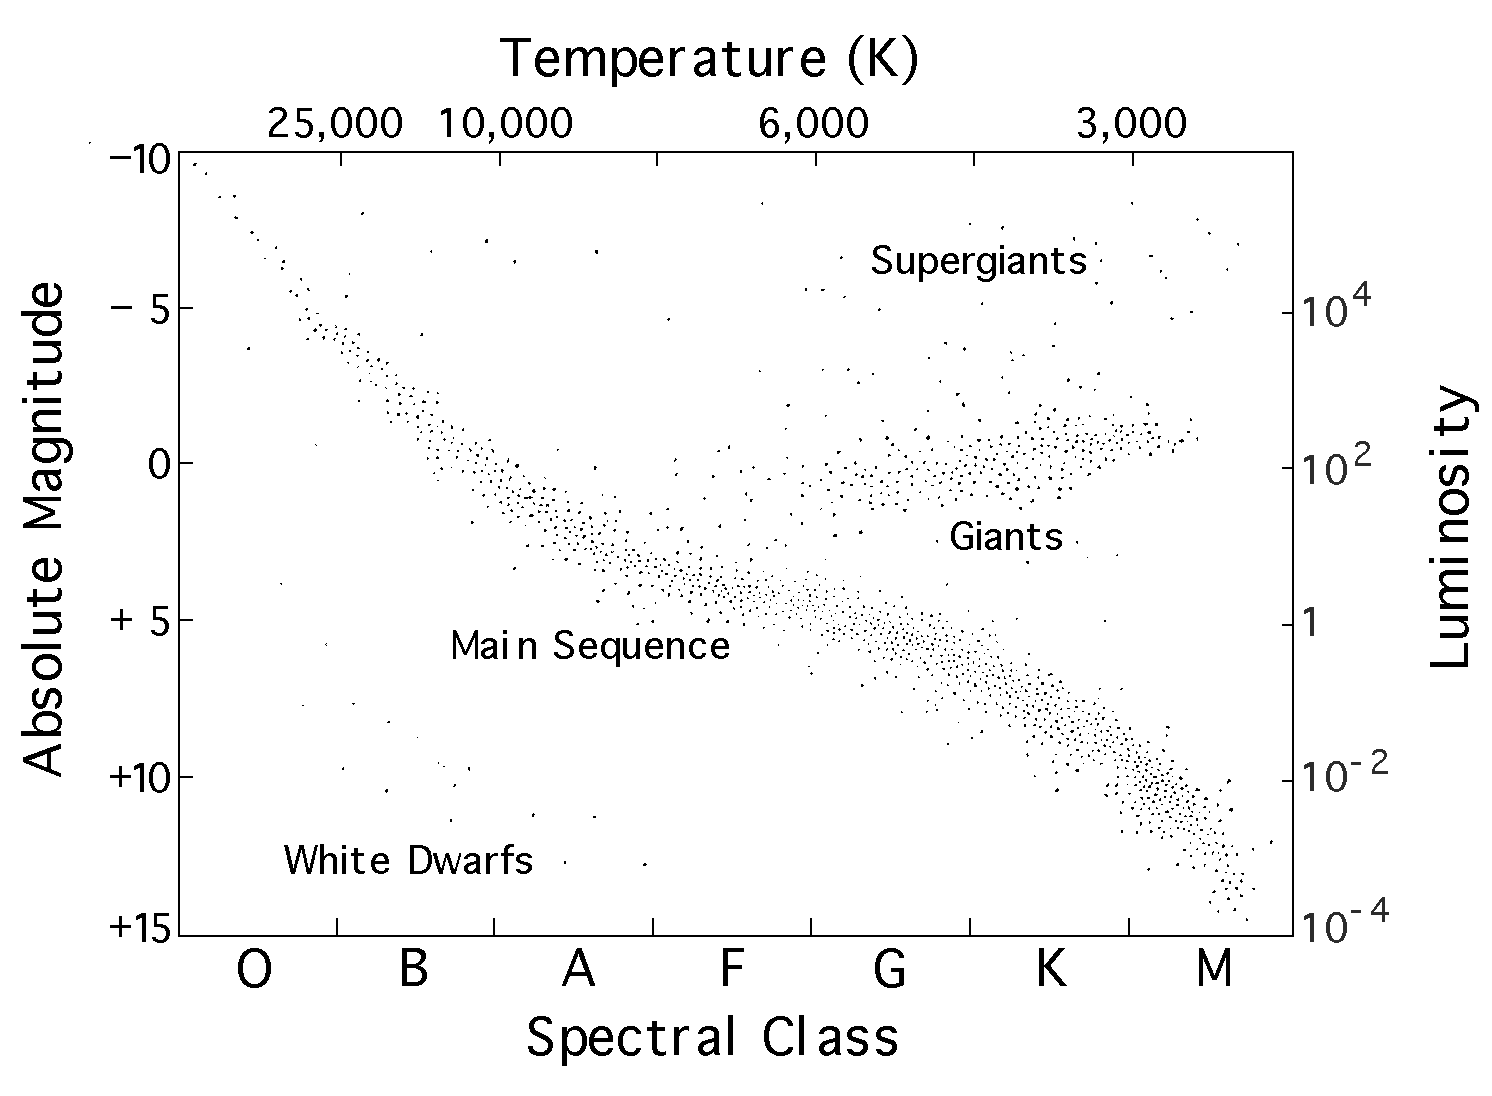
\includegraphics[scale=0.23]{../img/rus}
      \end{center}

      \begin{itemize}
        \item H 7 myr \
        \item He 500 kyr \
        \item C 600 yr \
        \item Ne 1 yr \
        \item Si 1 d \
        \item Core Collapse < 1s
      \end{itemize}

      \subsubsection*{Going Backwards}

      Also notice that if you go backwards along the plot, if we split up the large nucleons they will release energy as they go back up the potential. This is how we understand and make use of the energy in reactors. splitting $U$ for exmaple can give us over $200+ MeV$. 

      \subsection{TRIUMF}

      To figure out these binding energies, we can use something like TITAN and a beam of unstable nuclei. TITAN uses what we call a Penning Trap. It is a strong homogenous magnetic field and weak electrostatic field. By using the following equation we can accuratly measure the mass of the particle inside the trap.

      \[ v_c = \frac{1}{2\pi}\frac{q}{m}B\]

      The type of error we get is on the order of $10^{-12}$ enough to detect the $1\%$ changes in mass. TITAN is so accurate that if we were to weigh a plane, the error would be the mass of a missing screw.

      \subsection{Liquid Drop Model}
      \begin{defn}[Semi-empirical mass formula]\label{ldm}
      \[ E_b = a_V A-a_S A^{2/3} - a_C \frac{Z^2}{A^{1/3}} - a_A \frac{(A-2Z)^2}{A} - \delta(A,Z) \]
      Terms will be explained later...
      \end{defn}

      \subsection{The Valley}
      If we look at the isobars of a certain mass we can actually notice that mass vs z ha a very parabolic fit where the vertex also happens to be the most stable point. In fact, if you have a nucleid on the side of the valley, it will roll down the walls of the potential well by $p \rightarrow n$ or vise versa undergoing $\beta^{\pm}$ decay. At the tops of the valley are what we call drip lines. At the edges, the binding energy has gone to zero meaning that it is imposible to add more protons or neutons because they just drip away!


      \section{Nuclear forces and mesons}

      On the scale of atoms, the quantum effects are quite large. What we have to solve these kinds of problems is the schrodinger wave equation.

      \begin{defn}[Wave Equation]\label{swe}
        \[ -\frac{\hbar^2}{2m}\bigtriangledown^2\psi(r) + V(r)\psi(r) = E\psi(r) \]
      \end{defn}

      \subsection{Coulomb Force}
        Imagine a hydrogen atom where the coulomb potential of the proton was $V(r) = -ke^2/r$. When you solve the \nameref{swe} we can use what Planck discovered, $E=hf$ and get quantized spectral lines. This tells us that the electron and proton relationship is in fact a coulomb potential.

        At that time there was no evidence for any other forces effected the atom. However there clearly fould have be a force within the nuclei that attract the neutrons and protons that were very short range. Otherwise the protons would repel. 

      \subsubsection{Rutheford's Data}
        One way we tried to study it was to probe the nuclei with high energy protons. The scattering data as mentioned before is a way of sampling the fourier domain of the deflection from electrostatic repulsion. This was the equation predicted for the deflection with only the coulomb force..

          \[ p(\theta) = eQ^2 / e^2\sin^4(\theta/2) \]

        However with Rutheford's data, we were not able to find any difference between the evidence and the proposed results. Later on, with more energetic experiments, they could get the protons close enough to the nuclei that the short range force perturbed the predicted scattering.

      \subsection{Comparing Long and Short Range Forces}
        Understanding the nature of this short distance force can be best explained with comparing a long range force liek gravity with a short range force like the van de wals. 

        Consider the binding energy of a planet. The larger the planet the higher the excape velocity per unit mass. Now consider the energy it requies to vaporize a body of water. A cup, a bathtub, and ocean? It does not get any harder to boil the water per unit mass. 

        The same thing happens with the strong force. After say, $C^{12}$ the range of the force can only feel so many particles. That way after $C^{12}$ it becomes hard to really feel more particles. This is what \nameref{sat} is really about. In fact, we can actually use $C^{12}$ as a tough estimate for the range of the strong force, about $5fm$. It is actually more like $2-3 fm$
  
      \subsection{Probing the Nuclei}
        There are two techniques we use to study these kinds of properties. One is called scattering and the other is called bound state.

      \subsubsection*{Scattering}
        This is essentially what Rutheford did back in the day. We throw particles into a potential and see how the potential changes it's trajectory. By sampling $V(r)$ and finding it's inverse fourier transform, we can figure out the shape and amplitude of the potential.

      \begin{defn}[Born Approximation Scattering Amplitude]
      The scattering amplitude is the Fourier transform of the Scattering potential $V(r)$
        \begin{align*}
          A = \int \psi^{*}V(r)r\psi dr = \int e^{iqr}v(r)dr = fft(v(r))\
        \end{align*}
      \end{defn}

      \subsubsection{Bound State Spectrscopy}
      Just like atoms and molecules, nuclei exhibit a rich and complicated spectra of excited states, and these can tell us about the nuclear forces holding the nucleus together.

      \begin{align*}
        ^12C(\alpha,\gamma)^16O\\
      \end{align*}

      tigress an example of a bound state experiment. it can also measure posistion that lets us compensate for doppler effects in the experiment. 

      \begin{defn}[Parity]
        Tells whether the wavefunction is even or odd when $x \rightarrow -x$, wave functions are either even or odd functions. 
        \begin{align*}
          \Psi(-x) = \Psi(x) &\implies \pi = +1 \text{ even}\\
          \Psi(-x) = -\Psi(x) &\implies \pi = -1 \text{ odd}
        \end{align*}
      \end{defn}

      \subsubsection{Important Features of the Nuclear Binding Force}

      \begin{enumerate}
        \item Short-ranges (a few fm)
        \item Attactive at the distance > 0.6fm - that's what binds the nucleons together in a nucleus
        \item Strongly repulsive at short distances of < 0.5 fm - that's why nuclear matter is highly incompressible, and this causes the outward bounce. of the shock wave in a core - collapse supernova.
        \item \nameref{ssd} - quite unlike electromagnetic interactions in an atom or molecule.
        \item Doesn't distinguish between p - p, p - n or n - n, as long as they are in the same spin orientation.
      \end{enumerate}

      \subsubsection{Strong Spin Dependence}\label{ssd}

      Recall that protons and neutrons are spin $1/2$ particles. They have intrinsic angular momentum $1/2$ in units of $h / 2 \pi$. Relative to some direction z.

      Now consider the Deuteron. ($^2H$) It has a spin $J=1$ and consists of a protont and neutron with parallel spins with relative orbital angular momentum of $L=0$.If we try bond a proton and neutron with anti-parallel spins, the system will not bind together. It instantly falls apart.\\
      This is quite unlike the H atom, where the spin parallel and spin anti-parallel orientations result in a tiny splitting of the 1s level -- the origin of the 21 cm radio emission that radio astronomers use to map out hydrogen in the galaxy.\\
      Nuclear forces don't distinguish between protons and neutrons (neglecting the Coulomb interaction) as long as the two nucleons involved are in the same spin orientation. If the nuclear forces don't distinguish between protons and neutrons, then in some sense, we can regard protons and neutrons as two manifestations of the same particle.

      \begin{defn}[Nucleons and Isospin]\label{isospin}
        By analogy, nucleons are isospin-$1/2$ particles ($l=1/2$) with two possible isospin states, $l_3=+1/2$ for the proton and $l_3 = -1/2$ for the neutron.
      \end{defn}

      \subsection{Mesons}

      Later on the question became, 'what causes the nuclear forces?'. Yukawa made the analogy of fields in electromagnitism, charged partiles exchange photos to interact, since photons are massless, they have $\infty$ range. 

      In 1935, Yukawa proposed the meson, the photon equviliant of the strong force, Suppose that mesons have mass $m$, if a nucleon violates energy conservation to create a meson, we can use \nameref{hup} to calcuate the time it can last.

      \subsubsection{Yukawa Hypothesis}
      In the early 1930's it was know that the nuclear foces had a range of $\approx 2\text{fm}$ 

      Analogy with electromagnetism : Two chrages bodies do not interact by action at a distance but with an electric field ineracting with another body. This field can be quantized as photons with no mass and infinite range.\\
      In 1935 Yukawa postulated that the strong nuclear force is carried by quanta called mesons. Nucleons interacted by exchanging mesons.\\
      Supposed that the mesons have a mass $m$. Creating a energy violation with \nameref{hup} will result in 

      \[ \Delta t \le \frac{\hbar}{\Delta E} = \frac{\hbar}{mc^2}\]

      Since we know that a meson can travel a distance of $R = c\Delta t = \frac{\hbar c}{mc^2}$ using $\hbar c = 197.3 \text{MeV-fm}$ and knowing that $R \approx 2 \text{fm}$ we get that the mass should be around $100 \text{MeV}$. With the mass between electrons and nucleons there were called middle weight mesons.

      \begin{defn}[Yukawa Potential]\label{yp}
        The exchange of mesons of mass $m$ gives rise to a potential.
        \[ \Phi = ge^{\alpha r}/r \alpha = \frac{mc}{\hbar} \]
      \end{defn}

      In the limit $m\rightarrow0$ we get back the familiar coulomb potential.

      \[ \Phi = g \frac{1}{r} \equiv \frac{e}{4\pi\epsilon_0}\frac{1}{r}\]

      So we can think of $g$ as the "strong charge" giving rise to a meson potential $\frac{ge^{-\alpha r}}{r}$ in the same way that $e$ is the electric "electric charge" giving rise to an electric potential $\frac{e}{4\pi\epsilon_0}\frac{1}{r}$ The range of the Yukawa potential is approxixmately $\frac{1}{\alpha} = \frac{\hbar}{mc} = \frac{\hbar c}{mc^2}$, exactly what we got with the \nameref{hup} argument.\\
      In 1947 scientists went to the sky to look for cosmic rays for mesons using stacks of photographic. Usually, cosmic rays of protons around TeV colide with a nitrogen nuclous that break apart into pion -> muon + neutrino. 

      \subsubsection{From the Heisenberg uncertainty principle}
      The shorter the lifetime $\Delta t$ of a quantum state (such as a meson) the greater the uncertainty in its mass or energy $\Delta E$.

      \[ \Delta E \cdot \Delta t > h/2\pi\]

      So when these short-lived mesons are produced in a high energy particle collision, and you try to measure their mass, they show a width due to the uncertainty principle.
      The nucleus is a dynamic object where pions and heavier mesons constantly flit in and out of existence for only as long as permitted by \nameref{hup}. These temporary mesons that exist by energy borrowed from the uncertainty principle are called virtual mesons.

  %%%%%%%%%%%%%%%%%%%%%%%%%%%%%%%%%%%%%%%%%%%%%%%
  \end{document}
